\section{IoT System Architecture and Its Security Threat}
There are many framework architectures used in IoT system. The simplest and most well-known model is the three-layer model (figure \ref{fig:s2_3layer}): perception layer, network layer, application layer.  

\begin{itemize}
    \item \textbf{Perception Layer} or recognition layer: This layer’s main responsibility is to percept useful data from environment, translate those analog data into digital and send the data to the server.  The devices in this layer are: WSN node, RFID label, smart sensor. (We mentioned the threats of perception layer in section \ref{S2:SMARTDEVICE})
    \item \textbf{Network Layer} : The network layer of IoT is established on top of current internet structure. Its main features are conveying collected data, processing data and also providing a storage to those data. Because of its long history, the security status of this layer is relatively safe. However, threats like computer virus, network congestion causing the latency or unavailable in the system, Man-in-the-Middle attack can occur, and security mechanism is something that should not be ignored \parencite{STAGE:6188257}.
    \item \textbf{Application Layer} : The application layer uses the precepted data to create services. The range of services which IoT can provide are impressive: authentication, real time data visualization, smart house, smart building, automatic temperature controller and more. The main threat in this layer is the application itself. A software implemented by ignorant developers can be exploited to invade user’s privacy, cause damage to IoT devices or even harm users \parencite{STAGE:6188257}.
\end{itemize}

\begin{figure}
    \centering
    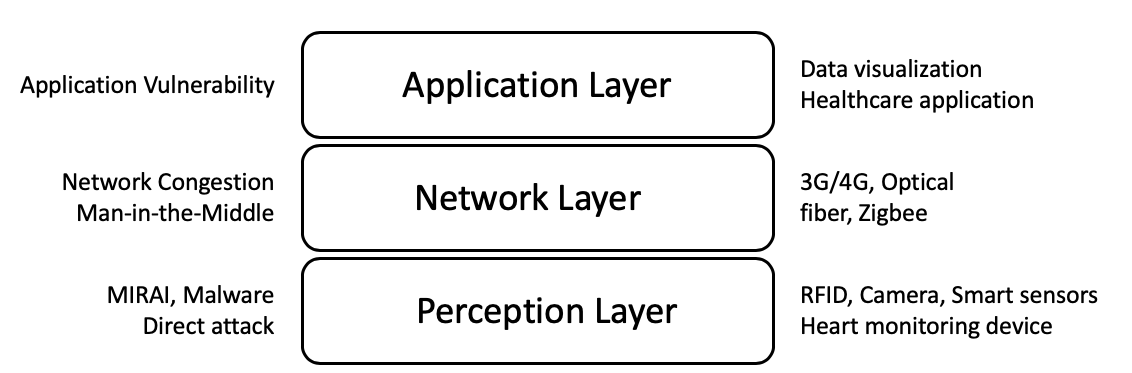
\includegraphics[width=0.7\textwidth]{1_3layer}
    \caption{3-layers Architecture}
    \label{fig:s2_3layer} 
\end{figure}

\section{Smart Device}
\label{S2:SMARTDEVICE}
Smart device is an electronic device, connected to other devices or networks. It is generally deployed at the perception layer of IoT system and used for collecting environment data or performing task from the command center. The characteristics of smart device can be summarized as below: 

\begin{itemize}
    \item \textbf{Deployed into the physical environment:} For example, electricity consumption meter is placed around electric cable to tracking how much electricity spent. Temperature meter embedded into the wall. Tsunami detection sensor located along the sea course. These devices are vulnerable to direct-attack. For example, using USB cable to connect into the system, and installing malicious software. 
    \item \textbf{Expected to operate without user’s recognition:}     After the initialization, devices are often deployed sparsely into outdoor environment. Normally, if no unexpected behavior has occurred, devices are simply left there without any attention.
    \item \textbf{Low computational power:}     In order to reduce the manufactured cost, these devices can only operate with a very limited set of functions. For example, smart sensor has only sensing and transmitting function. The device's computational power is insufficient to perform task like encryption. 
    \item \textbf{Communicate with a limited number of hosts:} IoT Smart device is different from our daily smart widget, it only needs to communicate with host we specified. 
\end{itemize}

\section{Whitelist and Blacklist}
Whitelisting and Blacklisting are network filtering techniques. Blacklist is a list contained with IP or domain name of malicious hosts, while whitelist is a list of secured hosts. A whitelist filter would allow all hosts from its list to communicate with device's network. A blacklist filter drops all packet from its list.  

Blacklist is normally used, when there is no specific communication pattern in the traffic. However, when communication pattern can be identified, it is more efficient to use whitelist.

The filtering is normally performed at layer 3 of the network, on the router. The wellknown firewall uses blacklist as its filtering protocol.


\section{Related Researches}
The security issues of IoT system arise from its heterogeneous nature. There was a time when IoT was developed with neither actual definition nor the standard. The companies which foresee the prosperity of IoT industry, developed and provided services as fast as they can, without paying much attention on the security system. The challenges of securing IoT are various: Authentication, Privacy protection, Access control, Cryptosystem and Security protocol, Software Vulnerability, Malware protection \cite{ISSUE1}\cite{ISSUE2}. 

A well implemented authentication method can help securing the privacy of IoT system, while protecting the integrity of data. Many researchers have tried to create a proper authenticate system for IoT system. M. Saadeh \textit{et al.}\cite{AUTH1} have classified authentication methods into 4 categories: Centralized, Distributed, Hierarchical and Flat. Each method has its own benefit, the selection of authenticate system depends on which kind of attack user wish to hinder. However, authentication do not focus on the security of the device, hence it would not work if the authenticated devices are compromised by adversaries. The hacked devices can still authenticate into the server and add any data. 

 The main concern about IoT system is the privacy. We place these smart devices closer to ourselves than any other kind of devices: from smart watch, security camera to even heart rate monitoring. The privacy breach, data leakage, is something that cannot allow to happen. G. Kalogridis \textit{et al.} \cite{PRIVACY1} have proposed a model to hind the electric consumption data in smart mater, while T. Song \textit{et al.} \cite{PRIVACY2} have introduced a scheme of data transmission with chaotic-generated symmetric key and secret key, guaranteeing the confidentiality and integrity. The privacy preserving data aggregation scheme has been presented by P. Yang \textit{et al.} \cite{PRIVACY3}, their approach can protect the privacy of data even when compromised nodes are available in the system.  

 With the heterogeneous nature of IoT system, it seems implausible to create the system which can protect IoT system from all possible attack surfaces. 
 C. Liu \textit{et al.} \cite{OTHER1} challenged this believe, and proposed that IoT security system should have an adaptive feature like immunity system. They have proposed a model which deal with the security threats according to its detector.
 J. Pacheco and S. Hariri \cite{OTHER2} also came up with a similar idea. They have inspected smart house/smart building sensor’s transmitted data, then used Anomaly Behavior Analysis (ABA) to identify the abnormality and perform the right recovery actions.  

 Most of previous researches seem to focus on data confidentiality, while left the integrity and the availability unresolved. We believe that the key to improving IoT system's integrity and availability is lied within the IoT device. Hence, in this reaseach, we  want to contribute in the improving of IoT security by finding a way to secure IoT devices. 

 